\section{Theorie}
\label{sec:theorie}

Heat capacity 
\begin{equation}
    C = \frac{\Delta Q}{\Delta T}
    \label{eq:heat_capacity}
\end{equation}
is described as the amount of heat energy $\Delta Q$ that is needed to heat up a probe by the temperature $\Delta T$.
With the first law of thermodynamics it is then possible to describe the amount of heat $\Delta Q$ in a more accurate way.
The first law of thermodynamics states 
\begin{equation*}
    \symup{d}Q = \symup{d}U + p\symup{V}
\end{equation*}
the infinisemal amount of heat $\symup{d}Q$ equals the inner energy $\symup{d}U$ added by the work done by the system or on the system.
Now two different heat capacities derive from the equation \eqref{eq:heat_capacity} depeding on the circumstances.
If the probe is heated up while its volume stays the same $\symup{d}V=0$ the heat capacity will be 
\begin{equation}
    C_\text{V} = \frac{\symup{d}U}{\symup{d}T}
    \label{eq:heat_cap_v}
\end{equation}
which is easy to calculate, but hard to measure.
If the probe is heated up by constant pressure the calculations will be harded but it is easier to measure the heat capacity as the heat expension or contraction does no matter.
To calculate the heat capacity at constant pressure $c_\text{p}$ from the heat capacity a constant volume $c_\text{v}$ the formula
\begin{equation}
    c_\text{p} - c_\text{v} = TVB\alpha_\text{V}^2
    \label{eq:correction_formula}
\end{equation}
can be used.
It contains the bulk module 
\begin{equation*}

\end{equation*}
and the kompression module
\begin{equation*}
    \, .
\end{equation*}
\subsection{Dulong-Petit}
As already mentioned the easiest way to calculate the heat capacity of a probe is to assume a constant volume.
By doing so just the inner energy needs to be derived by the temperature $T$.
In the classical model the inner energy
\begin{equation*}
    U = \frac{f}{2}Nk_\text{B}T
\end{equation*}
with $f$ being the degrees of freedom, $N$ the number of atoms, $k_\text{B}$ the Boltzman constant and $T$ the temperature.
The classical model assumes that the heat capacity is given by the amount of ozsillating atmos $N$ inside the probe.
Because the atoms can ozsillate into three directions, they have $f=6$ degrees of freedom.
This means the heat capacity at constant volume can be written as 
\begin{equation*}
    c_\text{v} = \frac{\symup{d}U}{\symup{d}T} = 3Nk_\text{B}
\end{equation*}
which further simplfies to the law of Dulong-Petit
\begin{equation}
    c_\text{v,mol} = 3R
    \label{eq:dulong}
\end{equation}
if we plug in the avogardo constant $N_\text{A} = N$ for the number of atoms and write $R = N_\text{A} k_\text{B}$, with $R$ being the gas constant.
The law of Dulong-Petit is a good approximation for some metalls at high temperatures above $T = \SI{300}{\K}$.
However it loses its accuracy for lower temperature at which the influence of quantum effects can not be neglected anymore.
\subsection{Einstein model}
As already mentioned the classical model breaks apart at low temperatures.
This is due to the impossibility of lattice ozsillations, which are called phonons, to take any energy level.
Similar to the harmonic oszillator, phonons can just take on discrete energys
\begin{equation}
    E_n = (n +\frac{1}{2})\bar{h}\omega
\end{equation}
with $n$ being a natural number called the occupation number, $\omega$ being its eigenfrequency and $\bar{h}$ being the reduced Planck constant.
As their energy $\bar{h}\omega>>k_\text{B}T$ becomes bigger than the energy given by the temperature they can not promote to a different energy level.
This behaviour is illustrated in figure \ref{fig:energy_phonon}.
\begin{figure}
    \centering
    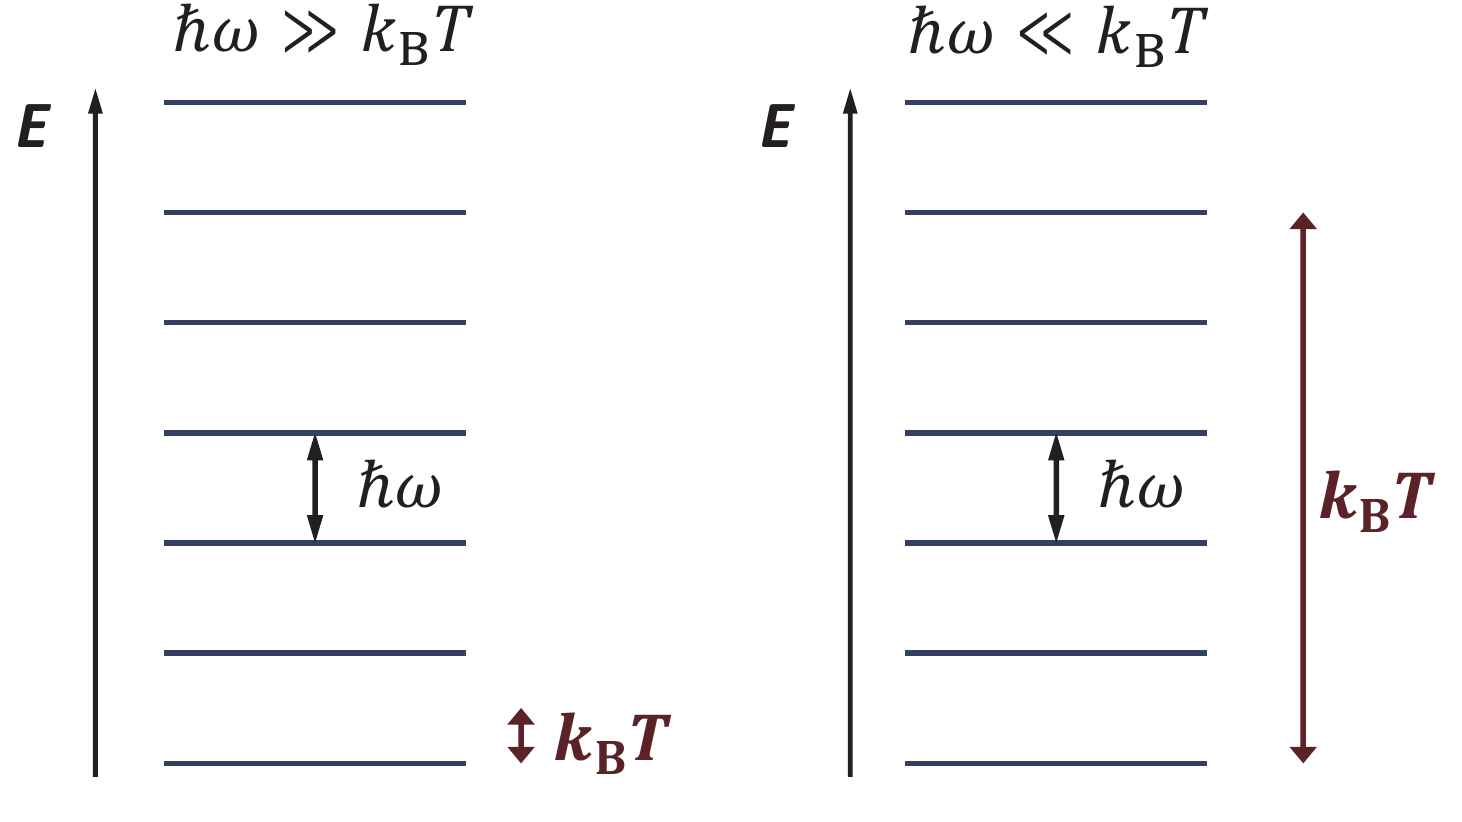
\includegraphics[width=\textwidth]{pictures/energy.png}
    \caption{The picture illustrates the impossibility of a phonon to absorb heat energy as the temperature lowers beneath the possible energys that the phonon can take on.}
    \label{fig:energy_phonon}
\end{figure}
Because of the quantized nature of phonon energy the averaged inner energy $<U>$ becomes
\begin{equation}
    <U> = U_\text{eq} + 3N\bar{h}\omega(\frac{1}{2} + <n>)
    \label{eq:inner_energy}
\end{equation}
where $U_\text{eq}$ is the inner energy in equilibrium.
One model that takes the quantum effects into account is the Einstein model.
In this model all the phonon modes are given the same possible eigenfrequency $\omega_\text{E}$.
With this assumption the averaged inner energy 
\begin{equation}
    <U> = 3N\bar{h}\omega_\text{E} \left ( \frac{1}{2} + \frac{1}{\symup{e}^{\bar{h}\omega_\text{E}/k_\text{B}T} - 1}\right )
\end{equation}
can be calculated by equation \eqref{eq:inner_energy}.
The heat capacity in the Einstein model is now calculate by equation \eqref{eq:heat_cap_v}.
The substitution 
\begin{equation}
    \Theta_\text{E} = \frac{\bar{h}\omega_\text{E}}{k_\text{B}}
\end{equation}